\section{When Is Instance Normalization Useful?} \label{ablation-studies}

\subsection{Controlled benchmark} \label{quantitative}

\paragraph{Compared components.}
We compare no normalization, global standardization, non-affine instance
normalization, and affine RevIN. For the two instance-normalized variants, we
also compare data-space MSE with normalized MSE,
\begin{equation}
 \mathcal{L}_{\mathrm{nMSE}}(\hat y,y\mid x)
 =\frac{1}{H}\sum_{h=1}^{H}
 \left(\frac{\hat y_h-y_h}{\sigma_x+\epsilon}\right)^2.
\end{equation}
Predictions are always returned to data space and evaluated with ordinary MSE;
normalized MSE only changes the weight assigned to each training window. This
factorial comparison separates the forward normalization, RevIN's affine
parameters, and scale-balanced optimization.

\paragraph{Datasets and splits.}
The expanded benchmark uses \textsc{ETTh1}, \textsc{Electricity},
\textsc{Traffic}, \textsc{Solar}, \textsc{Weather}, and
\textsc{Exchange Rate}. Dates are split sequentially into train, validation,
and test periods. Series are independently split into seen and unseen groups.
Models are trained on seen series in the training period and evaluated on
future dates for seen series (Test1) and future dates for unseen series (Test2).
We study $(L,H)$ in
\[
\{(168,24),(168,168),(504,24),(504,168),(504,504),
  (720,168),(720,720)\}.
\]

\paragraph{Protocol.}
We use \textsc{PatchTST} \citep{patchtst} and \textsc{DLinear}
\citep{dlinear}. Training samples random users and window starts, uses Adam
\citep{adam}, batch size 256, learning rate $10^{-5}$, and five seeds.
Every run uses exactly 10,000 optimizer steps. Validation is evaluated every
1,000 optimizer steps; evaluation windows use a
horizon-sized stride. Every table reports seed mean $\pm$ sample standard
deviation, while run summaries retain the variance and count of per-point loss
contributions. The rewritten implementation is first checked in short test mode
and then compared with the earlier results before the expanded analysis is
used.

% The bundled table is the previous three-dataset reproduction target. Once the
% new full run is complete, replace it with the generated mean-plus-uncertainty
% tables under outputs/revin_experiment/.
\begin{table}[t]
\caption{Ablation of RevIN components on \textsc{PatchTST} (MSE on new dates). Average improvements are reported relative to the no-normalization baseline. BP stands for ``backpropagation", Std. for "standard". In bold: best models per settings (rows).}
\centering
\setlength{\tabcolsep}{1.5pt}
\begin{tabular}{lccccccc}
\toprule
& & & & \multicolumn{2}{c}{RevIN (w/o $\alpha,\beta$)} & \multicolumn{2}{c}{RevIN} \\
     \cmidrule(r){5-6} \cmidrule(r){7-8}
 & L-H & None & Std. norm. & \thead{Std.\\BP} & \thead{Norm.\\BP} & \thead{Std.\\BP} & \thead{Norm.\\BP} \\
\midrule
\multirow{4}{*}{Electricity} & 168-24 & 349.83 & 20.56 & 8.52 & \textbf{4.91} & 8.52 & 4.92 \\
 & 504-24 & 348.14 & 19.68 & 8.36 & \textbf{4.09} & 8.34 & 4.09 \\
 & 504-168 & 347.21 & 28.28 & 11.00 & \textbf{7.09} & 10.94 & \textbf{7.09} \\
 & 504-504 & 358.70 & 33.18 & 16.70 & 12.54 & 16.65 & \textbf{12.53} \\
\midrule
\multirow{4}{*}{Solar} & 168-24 & 3.05 & 2.30 & 1.47 & \textbf{1.46} & 1.47 & 1.47 \\
 & 504-24 & 3.12 & 2.16 & 1.44 & \textbf{1.38} & 1.44 & 1.38 \\
 & 504-168 & 2.81 & 3.19 & 2.22 & \textbf{2.18} & 2.22 & \textbf{2.18} \\
 & 504-504 & 2.82 & 3.55 & 2.40 & \textbf{2.33} & 2.40 & \textbf{2.33} \\
\midrule
\multirow{4}{*}{Traffic} & 168-24 & 15.74 & \textbf{6.96} & 8.10 & 8.07 & 8.10 & 8.07 \\
 & 504-24 & 19.62 & \textbf{6.44} & 7.52 & 7.47 & 7.52 & 7.47 \\
 & 504-168 & 19.85 & \textbf{7.10} & 8.39 & 8.36 & 8.38 & 8.35 \\
 & 504-504 & 19.10 & \textbf{7.17} & 8.49 & 8.47 & 8.48 & 8.47 \\
\midrule
\multirow{3}{*}{Synthetic} & 40-10 & $3.4\times10^{6}$ & $1.5\times10^3$ & 4.28 & \textbf{4.27} & 4.28 & \textbf{4.27} \\
 & 100-20 & $3.2\times10^{6}$ & $5.3\times10^{3}$ & 3.66 & 3.66 & \textbf{3.65} & \textbf{3.65} \\
 & 100-100 & $3.2\times10^{6}$ & $9.8\times10^{3}$ & \textbf{4.25} & \textbf{4.25} & \textbf{4.25} & \textbf{4.25} \\
\midrule
Improvements &  & 0.0 $\%$ & 62.32 $\%$ & 70.1 $\%$ & \textbf{70.84} $\%$ & 70.11 $\%$ & 70.84 $\%$ \\
\bottomrule
\end{tabular}
\label{tab:main1}
\end{table}

\begin{table}[t]
\caption{Ablation of RevIN components on \textsc{PatchTST} (MSE on new dates and new users). Average improvements are expressed relative to the first column. BP stands for ``backpropagation", Std. for "standard". In bold: best models per settings (rows).}
\centering
\setlength{\tabcolsep}{1.5pt}
\begin{tabular}{lccccccc}
\toprule
& & & & \multicolumn{2}{c}{RevIN (w/o $\alpha,\beta$)} & \multicolumn{2}{c}{RevIN} \\
     \cmidrule(r){5-6} \cmidrule(r){7-8}
 & L-H & None & Std. norm. & \thead{Std.\\BP} & \thead{Norm.\\BP} & \thead{Std.\\BP} & \thead{Norm.\\BP} \\
\midrule
\multirow{4}{*}{Electricity} & 168-24 & 61.16 & 23.55 & 0.93 & \textbf{0.59} & 0.93 & \textbf{0.59} \\
 & 504-24 & 60.82 & 22.32 & 0.92 & \textbf{0.52} & 0.92 &\textbf{ 0.52} \\
 & 504-168 & 60.27 & 21.33 & 1.02 & \textbf{0.67} & 1.01 & \textbf{0.67} \\
 & 504-504 & 60.82 & 23.04 & 1.23 & \textbf{0.87} & 1.22 & \textbf{0.87} \\
\midrule
\multirow{4}{*}{Solar} & 168-24 & 2.74 & 2.35 & 1.31 & \textbf{1.30} & 1.31 & \textbf{1.30} \\
 & 504-24 & 2.74 & 2.20 & 1.28 & \textbf{1.23} & 1.28 &\textbf{ 1.23} \\
 & 504-168 & 2.54 & 3.24 & 1.97 & \textbf{1.94} & 1.97 & \textbf{1.94} \\
 & 504-504 & 2.52 & 3.59 & 2.13 & \textbf{2.06} & 2.13 & 2.07 \\
\midrule
\multirow{4}{*}{Traffic} & 168-24 & 14.44 & \textbf{6.51} & 7.30 & 7.27 & 7.30 & 7.27 \\
 & 504-24 & 19.60 & \textbf{6.02} & 6.77 & 6.72 & 6.77 & 6.72 \\
 & 504-168 & 18.75 & \textbf{6.87} & 8.13 & 8.09 & 8.13 & 8.09 \\
 & 504-504 & 17.87 & \textbf{6.99} & 8.29 & 8.26 & 8.28 & 8.25 \\
\midrule
\multirow{3}{*}{Synthetic} & 40-10 & $3.6\times10^{6}$ & $1.5\times10^{3}$ & \textbf{4.30} & \textbf{4.30} & \textbf{4.30} & \textbf{4.30} \\
 & 100-20 & $3.3\times10^{6}$ & $5.6\times10^{3}$ & \textbf{3.68} &\textbf{ 3.68} & \textbf{3.68} & \textbf{3.68} \\
 & 100-100 & $3.3\times10^{6}$ & $1.1\times10^{4}$ & \textbf{4.30} & \textbf{4.30} & \textbf{4.30} & \textbf{4.30} \\
\midrule
Improvements &  & 0.0 $\%$  & 6.97 $\%$   & 70.62 $\%$   & \textbf{71.29} $\%$   & 70.63 $\%$   & \textbf{71.29} $\%$   \\
\bottomrule
\end{tabular}
\label{tab:main2}
\end{table}


\paragraph{Reproduction hypotheses.}
The previous implementation suggested three findings to verify rather than
assume. First, normalized-space training improved data-space MSE on the more
heterogeneous collections. Second, the learnable affine parameters added little
over non-affine instance normalization. Third, global standardization remained
better on \textsc{Traffic}. The expanded dataset, horizon, backbone, and seed
sweep tests whether these observations are stable or dataset-specific.

\subsection{Relating gains to heterogeneity} \label{qualitative}

Instance normalization directly removes variation in look-back location and
scale. If $\mathcal{P}_{\mathrm{train}}$ and
$\mathcal{P}_{\mathrm{test}}$ denote input-window distributions, its most
plausible benefit is therefore in settings with shifts such as
\begin{equation}
 \mathbb{E}_{x\sim\mathcal{P}_{\mathrm{train}}}[\mu_x]
 \neq \mathbb{E}_{x\sim\mathcal{P}_{\mathrm{test}}}[\mu_x],
 \qquad
 \mathbb{E}_{x\sim\mathcal{P}_{\mathrm{train}}}[\sigma_x]
 \neq \mathbb{E}_{x\sim\mathcal{P}_{\mathrm{test}}}[\sigma_x].
\end{equation}
This is only a limited form of distribution alignment: higher-order structure,
frequency content, and dynamics may still differ. Conversely, removing
$(\mu_x,\sigma_x)$ is harmful when absolute level or scale helps predict the
horizon.

As a descriptive diagnostic, we compute energy distance
\citep{smola2006maximum} between train and test inputs,
\begin{equation}
d^2_{\mathrm{energy}}(P,Q)=
\mathbb{E}_{P,P}[k(x,x')]+\mathbb{E}_{Q,Q}[k(y,y')]
-2\mathbb{E}_{P,Q}[k(x,y)],
\quad k(x,y)=-\lVert x-y\rVert_2.
\end{equation}
These distances and the t-SNE visualizations \citep{tsne} are computed in a
separate dataset-analysis notebook, independently of model training. They are
used to test association with forecasting gains, not as evidence of causality.

\begin{table}[t]
\caption{Previously computed energy distances between input distributions.
T and S vary time periods and series, respectively. Values will be recomputed
with the expanded benchmark splits.}\label{tab:distances}
\centering
\setlength{\tabcolsep}{3pt}
\begin{tabular}{lrrrrrr}
\toprule
& \multicolumn{2}{c}{None} & \multicolumn{2}{c}{Standard}
& \multicolumn{2}{c}{Instance}\\
\cmidrule(lr){2-3}\cmidrule(lr){4-5}\cmidrule(lr){6-7}
& T & S & T & S & T & S\\
\midrule
Electricity & 7.09 & 57.16 & \textbf{0.05} & \textbf{0.42} & 0.64 & 1.01\\
Solar       & 3.48 & 0.98  & 1.05 & 0.30 & \textbf{0.78} & \textbf{0.29}\\
Traffic     & \textbf{0.32} & 0.99 & 1.39 & 4.29 & 0.92 & \textbf{0.45}\\
\bottomrule
\end{tabular}
\end{table}

\begin{figure}[t]
\centering
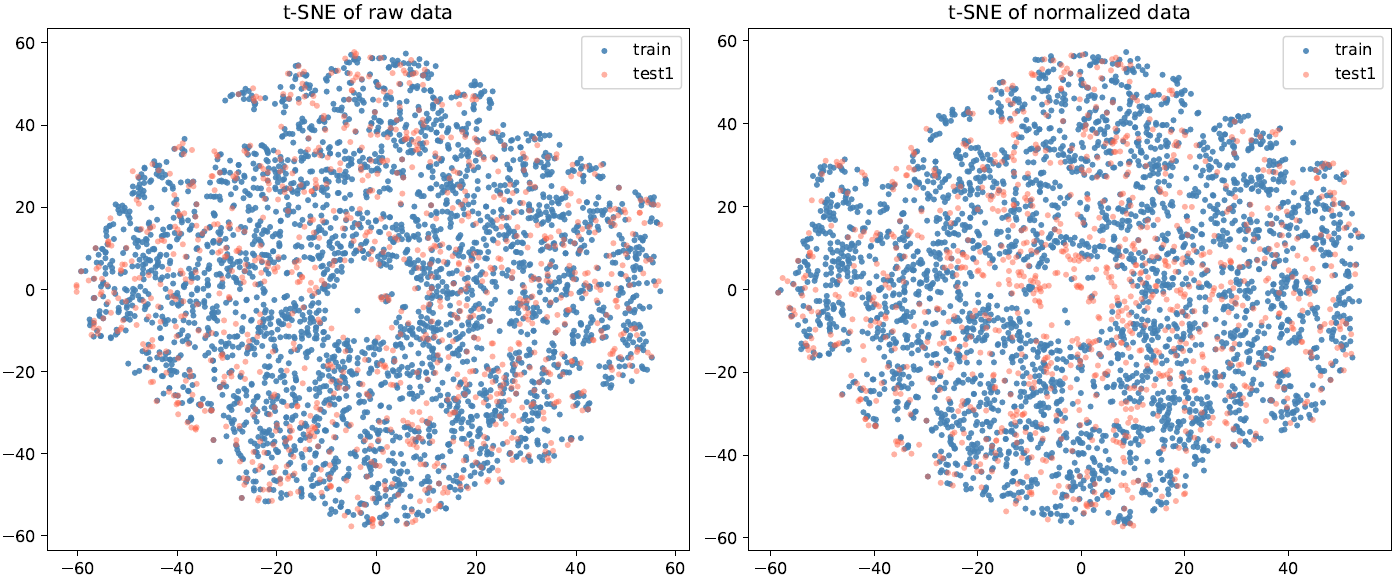
\includegraphics[width=0.7\linewidth]{Images/tsne/traffic_time_tsne.png}
\caption{Previous t-SNE embeddings of \textsc{Traffic} train (blue) and test
(orange) inputs before (left) and after (right) instance normalization.}
\label{fig:traffic_time_tsne}
\end{figure}

\subsection{Normalization choice as an oracle reference}

Raw MSEs are not directly comparable across datasets with different units. We
therefore report both the equal-configuration macro average
\begin{equation}
 \overline{M}(m)=\frac{1}{|\mathcal{C}|}
 \sum_{c\in\mathcal{C}}M_{c,m}
\end{equation}
and the mean per-setting relative gain over global standardization. In addition
to fixed standard, non-affine instance, and affine RevIN policies, we compute a
test oracle that chooses between standard normalization and full affine RevIN
for each dataset--setting pair. This oracle is an
optimistic upper reference, not a valid deployment procedure, because it uses
test outcomes for selection. Its gap to either fixed policy nevertheless
quantifies how much could be gained by learning a normalization-selection rule
from pre-test diagnostics. All policy comparisons use the same complete seeds
and report the standard deviation and variance of seed-level macro averages.
